\documentclass[a4paper,11pt]{article}

\usepackage[svgnames]{xcolor}
\usepackage{a4wide}
\usepackage{tikz}
\usetikzlibrary{arrows, pgfplots.groupplots}
\usepackage{pgfplots}
\pgfplotsset{compat=1.3}
\usepackage[detect-family]{siunitx}
\usepackage[eulergreek]{sansmath}
\sisetup{text-sf=\sansmath}
\usepackage{relsize}

\pagestyle{empty}

\begin{document}
% Based on station-layout.tex from Fokkema 2012.

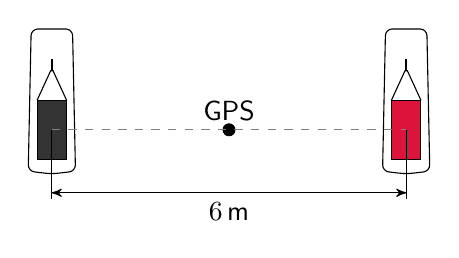
\begin{tikzpicture}
    [font=\sffamily, x=.75cm, y=.75cm,
     >=stealth',
%     thick,
    ]
    \foreach \sc / \col / \sx / \sy / \angle [count=\si] in
             {A/black!80!white/-3/0/180, B/Crimson/3/0/180} {
        \coordinate (\sc) at (\sx, \sy);
        \begin{scope}[shift={(\sc)}, rotate=\angle]
            % Skibox
            \draw[fill=white, rounded corners=2.25pt]
                (-.4, .7) .. controls (0, .75) ..  (.4, .7) --
                (.35, -1.7) .. controls (0, -1.72) ..  (-.35, -1.7) --
                cycle;
            % Scintillator
            \draw[fill=\col] (-.25, .5) rectangle (.25, -.5);
            % Lightguide
            \draw (-.25, -.5) -- (-.02, -1) --(.02, -1) -- (.25, -.5);
            % PMT
            \fill (-.02, -1) rectangle (.02, -1.2);
            % Detector number
            %\node[color=gray] at (-.75, -1) {\Large \si};
        \end{scope}
    }

    \coordinate (G) at (0, 0);
    % GPS
    \draw[fill] (G) circle (.10) node [above] {GPS};

    \coordinate (A'B) at ($ (A)!.8cm!-90:(B) $);
    \coordinate (B'A) at ($ (B)!.8cm!90:(A) $);
    \draw (A) -- ($ (A)!1.1!(A'B) $);
    \draw (B) -- ($ (B)!1.1!(B'A) $);
    \draw[<->] (A'B) -- (B'A) node [midway, below] {\SI{6}{\meter}};

    \draw[dashed,gray] (A) -- (B);
\end{tikzpicture}

\end{document}
